\section{Tempo}
\begin{osservazione}
In entrambi i casi, algoritmi paralleli e algoritmi distribuiti, la risorsa tempo è cruciale
\end{osservazione}

\paragraph{Come si misura il tempo?} Il tempo è misurato come la quantità di operazioni elementari richieste per risolvere il problema. 

\paragraph{Tempo nel caso sequenziale} 
$$t(n) = max\;\{T(x)\;|\;x \in \Sigma^n\}$$
In questo caso entra in gioco la definizione formale $T(x)$, è il numero di operazioni elementari che servono per risolvere il problema su un'istanza $x$, dove $x$ è l'input 

Si definisce $t(n)$ il $max$ tra tutti i $T(x)$ dove $x$ è un'istanza di lunghezza $n$. E' la valutazione $T(x)$ nel caso peggiore. E' una funzione in $n$, dove $n$ è la lunghezza dell'input

\begin{osservazione}
    Spesso non saremo interessati ad una valutazione precisa di $t(n)$, ma al suo tasso di crescita, ci basta valutare l'ordine di grandezza, il tasso di crescita della funzione. Per questo useremo le funzioni asintotiche  O,$\;\Omega, \;\Theta$
\end{osservazione}

\begin{figure}[h]
    \centering
    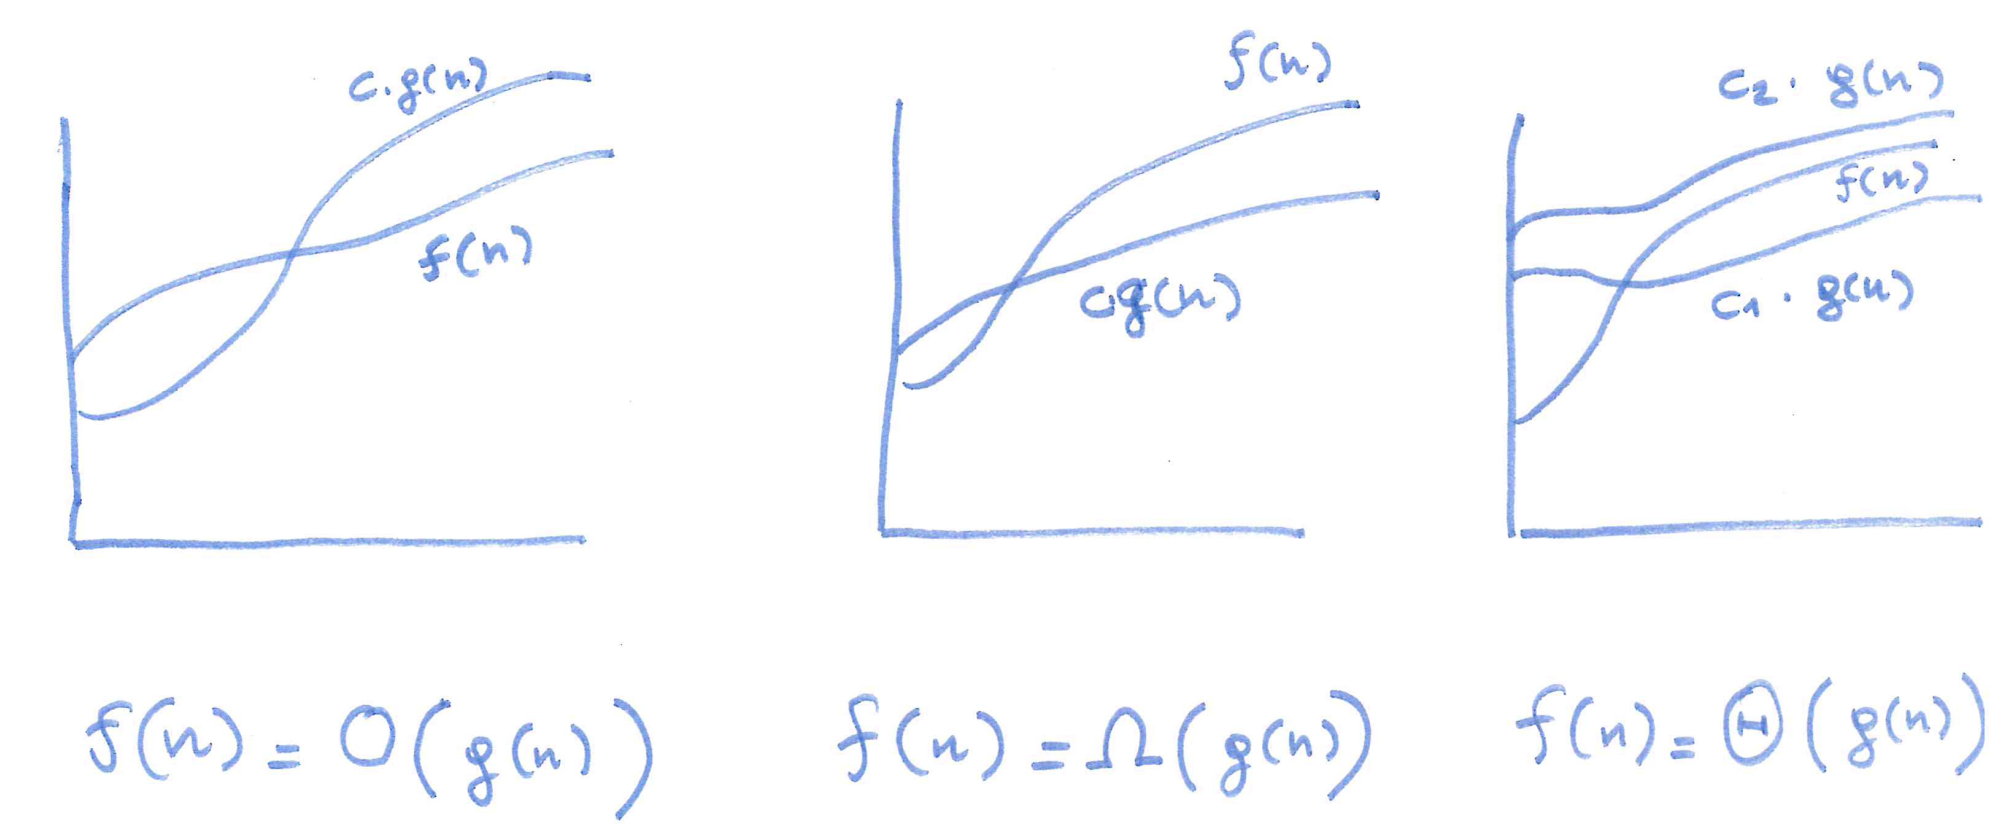
\includegraphics[scale=0.4]{images/funzioni_asintotiche.png}
    \caption{Funzioni asintotiche}
\end{figure}

Quindi O di $log_n$ vuol dire che non cresce più di $log_n$, è limitata superiormente dalla funzione $g(n)$. $\Omega(g(n))$ vuol dire che è limitato inferiormente, quindi può essere più grande di $g(n)$

\paragraph{Avvertenze sulla valutazione di t(n)}
\begin{itemize}
    \item $t(n)$ viene valutata su un particolare modello di calcolo. Quello che contiamo sono le operazioni elementari che il modello di calcolo ci offre
    \item Va scelto il \uline{criterio di costo: \textit{uniforme} o \textit{logaritmico}}. Se utilizzo il criterio di costo uniforme le operazioni elementari richiedono un'unità di tempo, se utilizzo il criterio di costo logaritmico considero le operazioni elementari ma ogni operazione ha un peso che è diverso a seconda della dimensione dei numeri che sono in gioco. Noi useremo il costo uniforme. Il costo logaritmico prende in considerazione anche la dimensione dei dati.
\end{itemize}

\paragraph{Teoria della complessità}
Possibili tassi di crescita di $t(n)$
\begin{itemize}
    \item logaritmico quando è $O(\log n)$
    \item polilogaritmico quando è $O(\log^k n)$ per una costante $k > 0$
    \item lineare quando è $O(n)$
    \item polinomiale quando è $O^k$ per una costante $k > 0$
    \item esponenziale quando NON è $O^k$ per ogni costante $k > 0$
\end{itemize}

\subsection{Concetto di efficienza}
Questa funzione tempo dovrà dirci se i nostri algoritmi sono efficienti.

\paragraph{Caso sequenziale}
Cosa era efficiente nel caso sequenziale? 

Un problema è risolto efficacemente in tempo sse è risolto da una Macchina di Turing deterministica in tempo polinomiale.

Tempo polinomiale $=$ efficienza, perchè? Perchè la classe di problemi risolta in tempo polinomiale (P, FP) risulta essere robusta rispetto a svariati modelli di calcolo. Finchè la funzione tempo è polinomiale i tempi sono ragionevoli, quando diventa esponenziale non vanno bene più.

\paragraph{Classi di problemi}
Quindi \textit{P} ed \textit{FP} hanno una definizione robusta che non cambia con il modello di calcolo. Purtroppo altri problemi interessanti non hanno ancora soluzioni efficienti e stanno in \textit{NP}: problemi di decisione risolti in tempo polinomiale su una Macchina di Turing non deterministica. Esempio la fattorizzazione di interi, utile per algoritmi di crittografia. 

I problemi in \textit{NP} sono quei problemi di cui non si sa se esiste un algoritmo polinomiale per essi.

L'efficienza nel caso parallelo è \textit{NC}. Ciò che si sa è che $NC \in FP$. Cioè se ho un algoritmo parallelo efficiente per un certo problema ho anche un algoritmo sequenziale efficiente e la cosa è vera perchè prendo l'algoritmo parallelo lo do ad un processore che esegue in sequenza le istruzioni del mio algoritmo parallelo. Siccome risulta essere efficiente nel caso parallelo, risulta essere efficiente anche nel caso sequenziale. Sono quei problemi risolti con algoritmi paralleli veloci, cioè tempo poli-logaritmico, ad esempio $log_4(n)$ o $log_3(n)$ e hardware polinomiale, anche l'hardware ha un limite superiore. Non possiamo dire che un problema viene risolto in modo efficiente nel mondo parallelo se utilizziamo ad esempio un hardware esponenziale, perchè risulta impraticabile per istanze anche molto piccole dell'input. I problemi che stanno in NC sono quelli altamente parallelizzabili che stanno in FP

$NC = FP$? Problema aperto, si pensa di no! Rispondere a questa domanda è come rispondere alla domanda: ogni algoritmo efficiente è parallelizabile (rimanendo chiaramente efficiente)?

Le classi di problemi P, FP, NP e NC sono classificazioni utilizzate per descrivere la complessità temporale degli algoritmi utilizzati per risolvere i problemi
\begin{itemize}
    \item La classe P (Polynomial) include tutti i problemi per i quali esiste un algoritmo di soluzione efficiente, ovvero che ha una complessità temporale polinomiale
    \item La classe FP (Functional Polynomial) include tutti i problemi per i quali esiste un algoritmo di verifica efficiente, ovvero che ha una complessità temporale polinomiale, ma per i quali non esiste un algoritmo di soluzione efficiente
    \item Per la classe NP non esiste un algoritmo di soluzione efficiente per questi problemi, ovvero con complessità temporale polinomiale  
    \item La classe NC (Non-deterministic Polylogarithmic) include tutti i problemi per i quali esiste un algoritmo di soluzione con complessità temporale poli-logaritmica
\end{itemize}



\newpage